\documentclass[tikz,border=8pt]{standalone}
% Shared look for every TikZ diagram. Load with \input{../../tools/tikz-style.tex}
\usepackage[T1]{fontenc}
\usepackage{lmodern}
\renewcommand{\sfdefault}{lmr}  % diagrams use the same serif as the text
\usetikzlibrary{arrows.meta, positioning, shapes.geometric, calc, fit, backgrounds}
\definecolor{cblue}{HTML}{4C78A8}
\definecolor{corange}{HTML}{F58518}
\definecolor{cgreen}{HTML}{54A24B}
\definecolor{cred}{HTML}{E45756}
\definecolor{cpurple}{HTML}{B279A2}
\definecolor{cgrey}{HTML}{6B6B6B}
\tikzset{
  every picture/.style={font=\sffamily, line width=1.2pt},
  box/.style={draw=#1, fill=#1!12, rounded corners=4pt, align=center, inner sep=7pt, minimum height=1.1cm},
  box/.default=cgrey,
  arrow/.style={-{Stealth[length=3mm]}, draw=cgrey, line width=1.4pt},
  title/.style={font=\sffamily\bfseries\Large},
  note/.style={font=\sffamily\small, text=cgrey, align=center},
}
\AtBeginDocument{\hyphenpenalty=10000 \exhyphenpenalty=10000}

\begin{document}
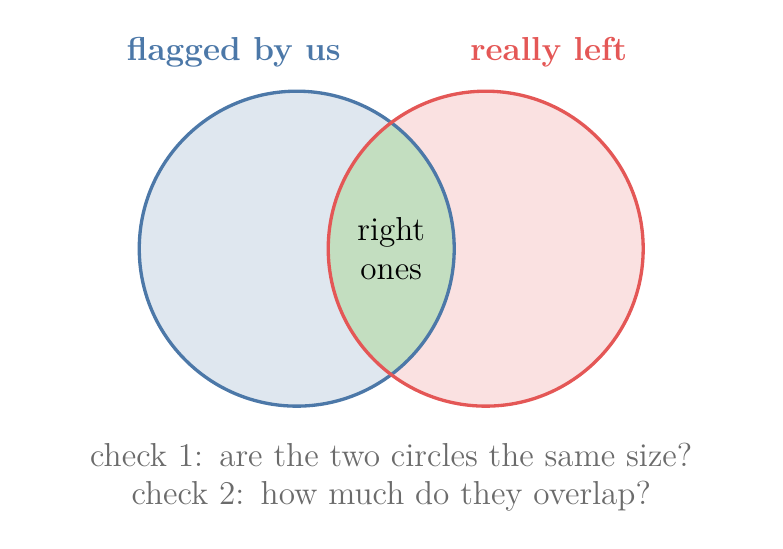
\begin{tikzpicture}[every node/.append style={font=\sffamily\large}]
\tikzset{note/.style={font=\sffamily\large, text=cgrey, align=center}}
  \fill[cblue!18] (0,0) circle (2.0);
  \fill[cred!18] (2.4,0) circle (2.0);
  \begin{scope} \clip (0,0) circle (2.0); \fill[cgreen!35] (2.4,0) circle (2.0); \end{scope}
  \draw[cblue] (0,0) circle (2.0);
  \draw[cred] (2.4,0) circle (2.0);
  \node[text=cblue, font=\sffamily\bfseries\large] at (-0.8,2.5) {flagged by us};
  \node[text=cred, font=\sffamily\bfseries\large] at (3.2,2.5) {really left};
  \node[align=center] at (1.2,0) {right\\ones};
  \node[note, text width=9cm] at (1.2,-2.9) {check 1: are the two circles the same size?\\check 2: how much do they overlap?};
\end{tikzpicture}
\end{document}
